\documentclass[11pt]{article}

\usepackage{fancyhdr}
\usepackage{graphicx}
\usepackage{geometry}
\usepackage{lastpage}
\usepackage{titling}
\usepackage{sectsty}
\usepackage{setspace}
\usepackage{changepage}
\usepackage[shortlabels]{enumitem}
\usepackage{subcaption}
\usepackage{helvet}
\usepackage{hyperref}

\usepackage{siunitx}
\usepackage{nicefrac}
\usepackage{amsmath}
\usepackage{gensymb}
\usepackage{amssymb}
\usepackage{float}
\setcounter{MaxMatrixCols}{11}

\usepackage{listings}
\usepackage{matlab-prettifier}
% \usepackage{color}
% \definecolor{dkgreen}{rgb}{0,0.6,0}
% \definecolor{gray}{rgb}{0.5,0.5,0.5}
% \definecolor{mauve}{rgb}{0.58,0,0.82}

\lstset
{
  frame=tb,
  style=Matlab-editor,
  % language=MATLAB, %Matlab-editor,
  aboveskip=3mm,
  belowskip=3mm,
  showstringspaces=false,
  columns=flexible,
  basicstyle={\small\ttfamily},
  numbers=none,
  % numberstyle=\tiny\color{gray},
  % keywordstyle=\color{blue},
  % commentstyle=\color{dkgreen},
  % stringstyle=\color{mauve},
  breaklines=true,
  breakatwhitespace=true,
  tabsize=3
}

\geometry
{
  letterpaper, 
  total={175.9mm,229.4mm}, 
  top=25mm, 
  left=20mm, 
  headheight=26pt,
  voffset=12pt,
  footskip=15pt
}
\author{Daniel Sturdivant}
\title{Lab 2}
\date{February 2023}
\graphicspath{ {./media/} }

\pagestyle{fancy}
\fancyhead[R]{February 27, 2023}
\fancyhead[L]{Sturdivant, Daniel \\ Weir, Andrew}
\fancyhead[C]{MECH 6970 Intro to GPS}
\fancyfoot[C]{Page \thepage\ of \pageref{LastPage}}

\makeatletter
\def\@maketitle
{
  \null
  \begin{center}
    {\huge \@title \\}
  \end{center}
  \vskip 5mm
}
\makeatother

\sectionfont{\fontsize{16}{16}}
\subsectionfont{\fontsize{13}{13}\normalfont}
\renewcommand{\thesubsection}{\arabic{section}-\arabic{subsection}}
\renewcommand{\familydefault}{\sfdefault}
\newcommand{\solution}{\textbf{Solution: \\}}


%% ====================================================================== %%
\begin{document}

\maketitle
\thispagestyle{fancy}
\setstretch{1.25}
% \setlength{\parskip}{0em}
% \setlength{\abovedisplayskip}{-8pt}
% \setlength{\belowdisplayskip}{12pt}
\setlength{\parindent}{0pt}

% PART 1
\begin{enumerate}[label=\textbf{\arabic*.}]
  \itemsep 24pt
  \item Using the RCVR\_S1 data from the class website: 
  \begin{enumerate}[(a)]
    \itemsep -2pt 
    \item Using the ephemeris, determine the SV positions as a function of GPS time. You can
    check your calculation using initial satellite positions provided. Provide a sky plot of the
    SV positions over the period of the data collection
    \item Using the pseudoranges and SV positions, calculate the GPS position. You can check
    your calculations using the initial GPS position provided.
    \item Convert the ECEF positions to LLA and plot in Google Earth, Google Maps, or GPS
    visualizer. Where was the data taken and how much error/wander does there appear to
    be over the static data set?
    \item Convert the ECEF positions from the Novatel to ENU (use Toomers Corner as the
    reference location). Plot the E,N,U positions vs. time and characterize their errors.
    Compare this to the DOP.
    \item Calculate and plot the velocity in ENU coordinates. What measurement did you use for
    velocity? What is the accuracy in each axis?
  \end{enumerate}
  \solution
  Satellite positions were determined by using the calc\_gps\_sv\_pos function 
  given on the class website. This function takes in given ephemeris data, a GPS 
  transmit time and a calculated transit time. The transit and transmit time were 
  calculated with the following equations:
  \begin{equation*}
    \begin{split}
      t_{transit} &= \dfrac{\rho}{c} \\
      t_{transmit} &= t_{GPS} - t_{transit}
    \end{split}
  \end{equation*}
  This results in the following skyplot:
  \begin{figure}[H]
    \centering
    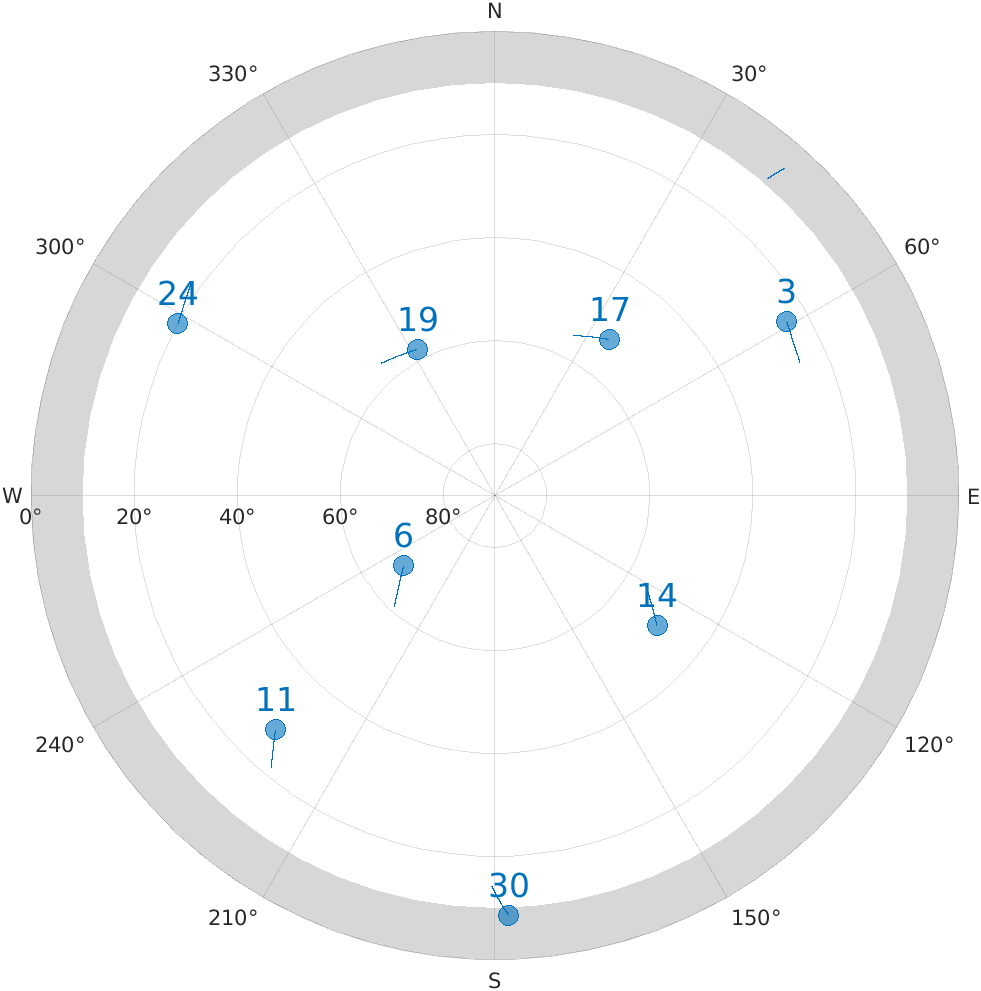
\includegraphics[width=0.6\textwidth]{static_skyplot.png}
    \caption{Static Receiver Skyplot.}
  \end{figure}
  The receiver position was calculated using a Gauss-Newton least squares 
  approach shown in the following code.
  \begin{lstlisting}
    function [x,b,P,DOP,i] = gnssPos(x_sv, psr, psr_var, x_hat)
    % get number of measurements
    N = size(x_sv, 1);
    % determine if weighted or unweighted least squares
    if length(psr_var) == 1
        W = eye(N);
        wgt = false;
    else
        W = inv(diag(psr_var));
        wgt = true;
    end
    % initial conditions
    if nargin < 4
        x_hat = [0;0;0;0];
    end
    error = Inf;
    i = 0;
    % least squares iterations
    while (error > min(psr_var.^2)*1e-3) && (i < 10)
    % while error > 1e-6
        i = i + 1;
        u = x_sv - x_hat(1:3)';
        r = sqrt(sum(u.^2,2));
        uv = u./r;
    
        H = [-uv, ones(N,1)];       % geometry matrix [-ux/r, -uy/r, -uz/r, 1]
        y = psr - (r + x_hat(4));   % meas. vector [rho - (r + b)]
        dx = inv(H'*W*H)*H'*W*y;
    
        x_hat = x_hat + dx;
        error = norm(dx);
    end
    x = x_hat(1:3);
    b = x_hat(4);
    % calculate covariance
    if wgt
        P = inv(H'*W*H);
    else
        P = psr_var^2 .* inv(H'*H);
    end
    DOP = inv(H'*H);
    end    
  \end{lstlisting}
  Using the code, an initial receiver position was found to be: 
  \begin{equation*}
    \begin{split}
      x \:\si{[m]} &= 
      \begin{bmatrix}
        422597.61 & -5362875.44 & 3415503.25
      \end{bmatrix} \\
      x \:\si{[\circ, \circ, m]} &=
      \begin{bmatrix}
        32.586296 & -85.494370 & 209.357
      \end{bmatrix}
    \end{split}
  \end{equation*}
  In the static data there was a time jump of about 5 minutes after 914 seconds. This itself 
  would not be an issue but there was an extra second added at index number 1067 which had 
  to be accounted for. Plotting the position output with these adjustments:
  \begin{figure}[H]
    \centering
    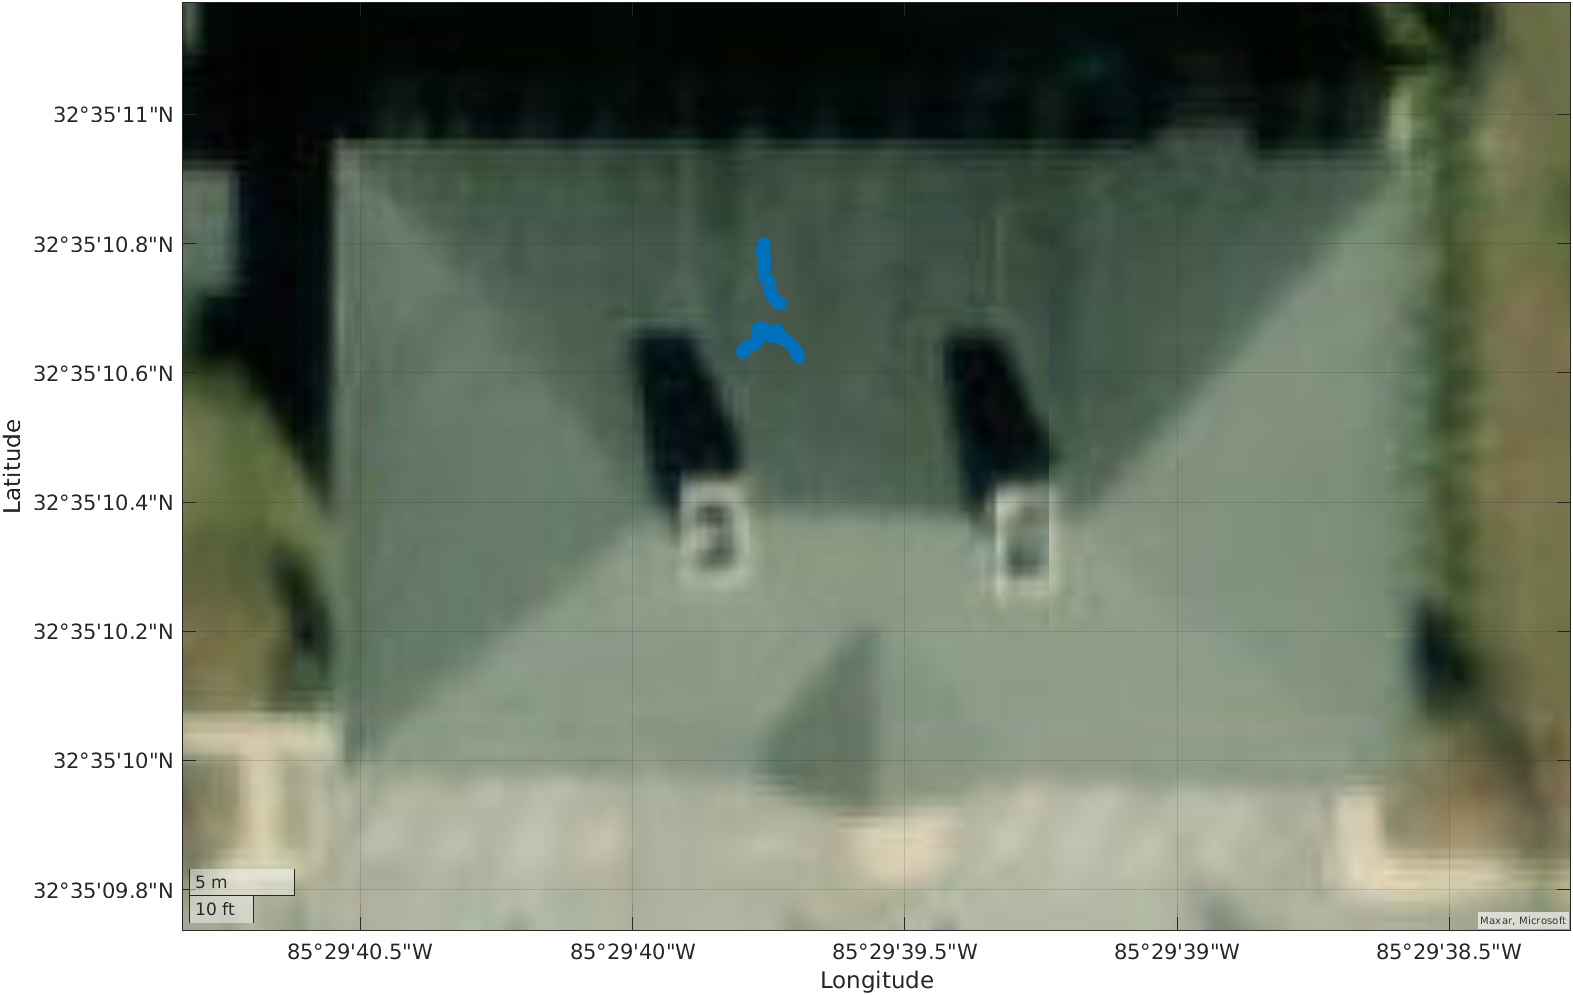
\includegraphics[width=0.7\textwidth]{static_pos.png}
    \caption{Positioning of the Static Receiver.}
  \end{figure}
  By looking at the geoplot it can be seen that the data was taken at the Auburn MRI 
  building. There does seem to be some wander on the position measurements, as 
  two line segments are formed by the position measurements drifting over time. 
  However, this drift is limited to less than a few meters of error. Exact ENU 
  positions were calculated with Toomer's Corner as a reference position. The position 
  jump between approximately 900 and 1200 seconds is also apparent.
  \begin{figure}[H]
    \centering
    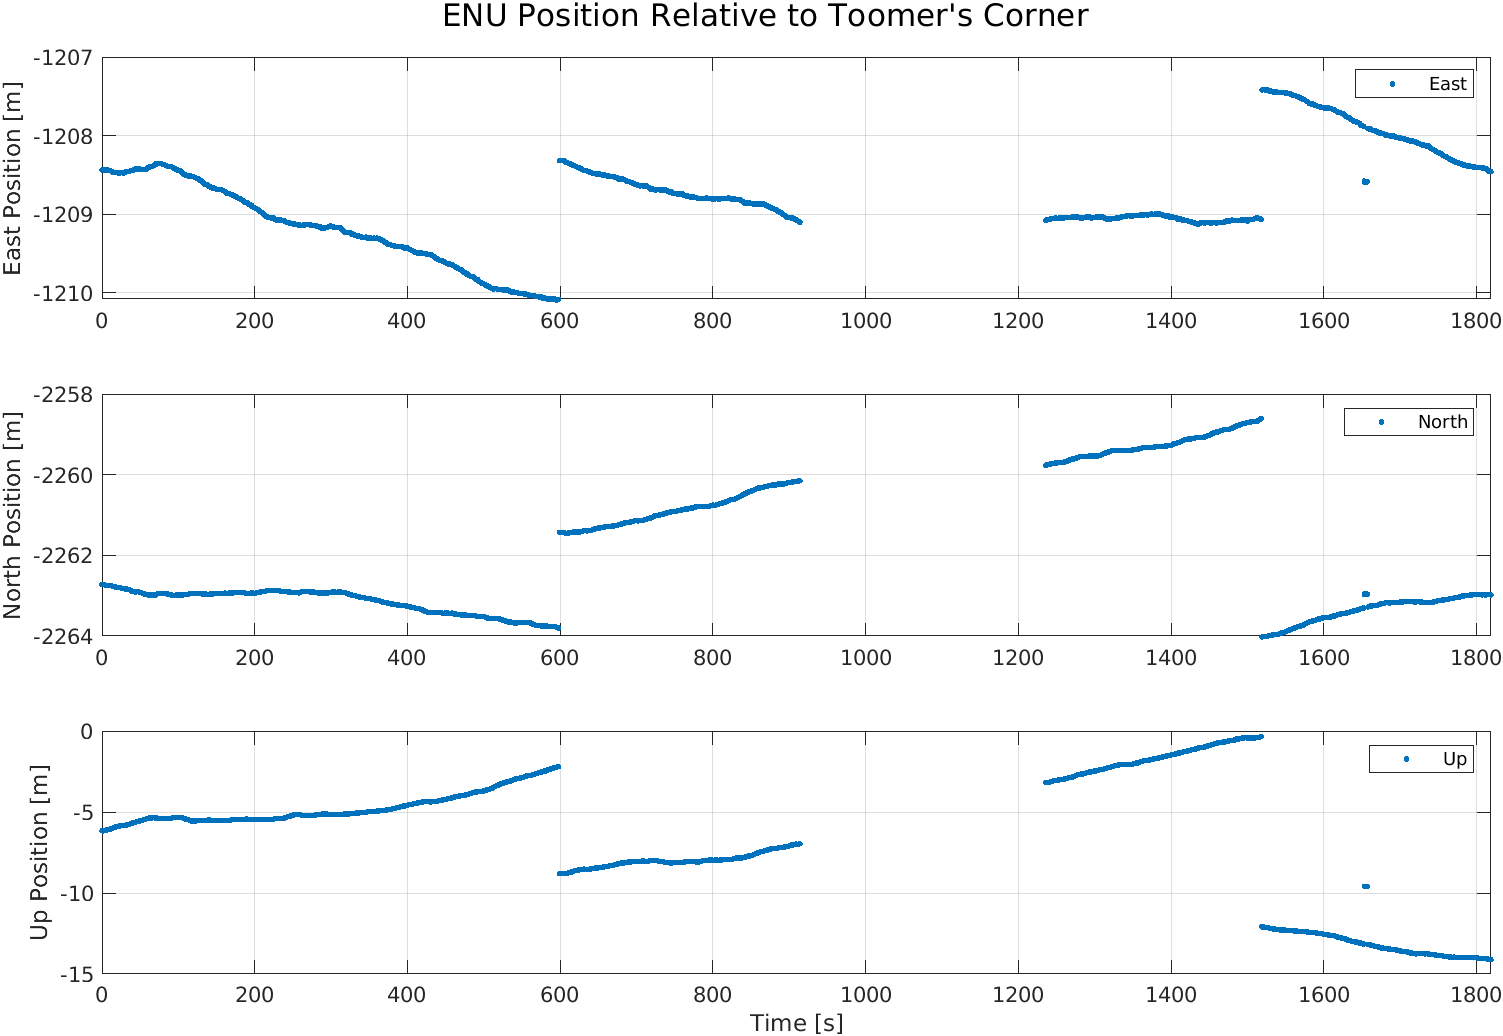
\includegraphics[width=0.7\textwidth]{static_pos_enu.png}
    \caption{ENU Position Relative to Toomer's Corner.}
  \end{figure}
  Based on the ENU positions it can be seen that the positions errors remain 
  less than a few meters until a satellite is lost at 600 seconds and again between 
  1400 and 1500 seconds. The plots of the DOP below also show this jump in position error.
  \begin{figure}[H]
    \centering
    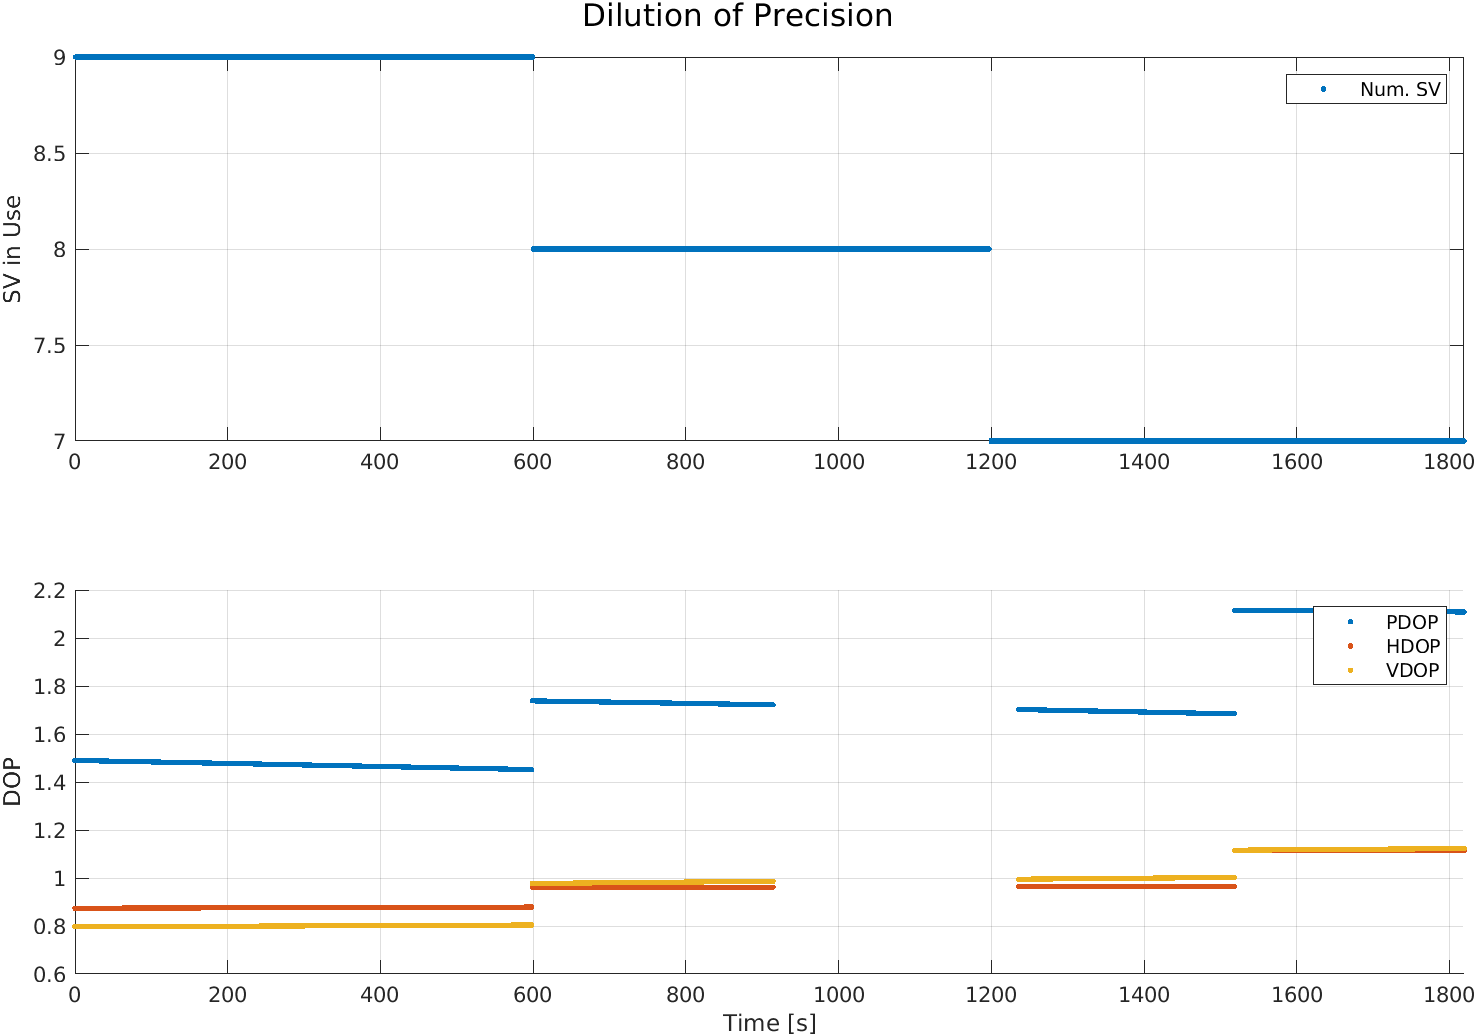
\includegraphics[width=0.7\textwidth]{static_dop.png}
    \caption{Static Receiver Dilution of Precision.}
  \end{figure}
  The PDOP shows that the position error be should held relatively constant. \\

  The following is a plot of the ENU velocities which again shows the time jump:
  \begin{figure}[H]
    \centering
    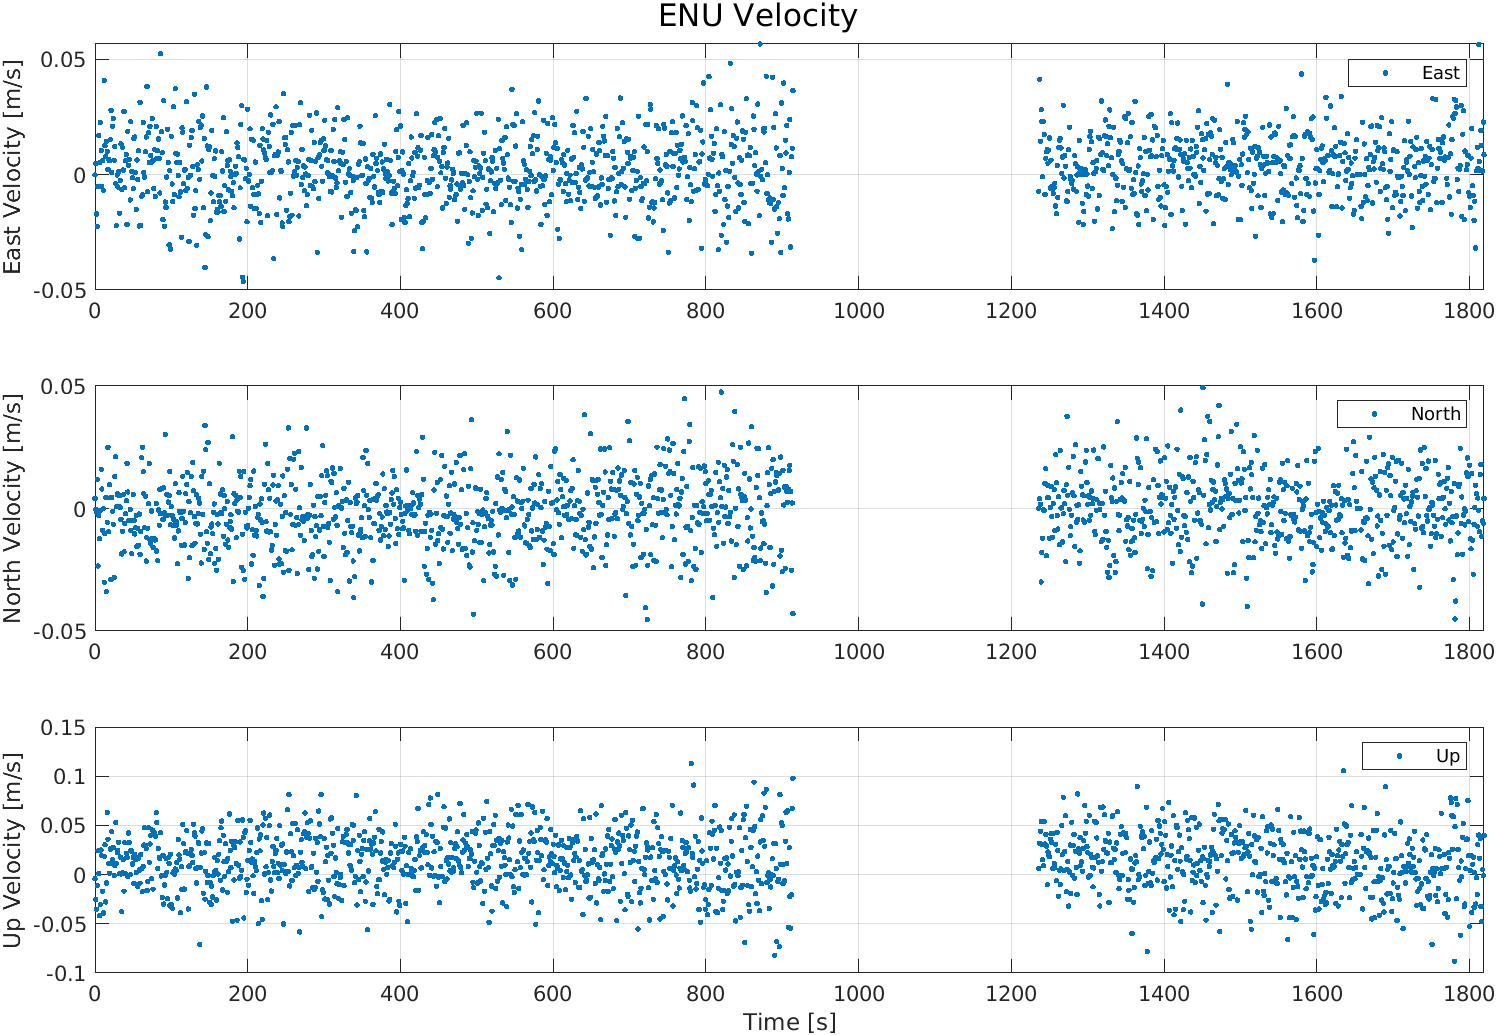
\includegraphics[width=0.7\textwidth]{static_vel_enu.png}
    \caption{ENU Velocity.}
  \end{figure}
  The ECEF velocities were calculated using the doppler measurements and 
  satellite velocities with a closed form least squares solution. 
  \begin{lstlisting}
    function [xDot, bDot] = gnssVel(x_sv, v_sv, x_user, dopp)
    N = size(x_sv, 1);
    % generate unit vector and range to satellite
    u = x_sv - x_user';
    r = sqrt(sum(u.^2,2));
    uv = u./r;
    % least squares parameters
    H = [-uv, ones(N,1)];
    y = dopp - sum(uv.*v_sv, 2);
    x = inv(H'*H)*H'*y;
    xDot = x(1:3);
    bDot = x(4);
    end    
  \end{lstlisting}
  The ECEF velocities were converted to ENU using the MATLAB function 
  \emph{ecef2enuv}. The ENU velocities for each axis are approximately 
  zero mean. For a majority of the run, the accuracy at each axis is below 
   a magnitude of 0.05 meters per second. 

  \item Using the RCVR\_D1 dynamic data from the class website:
  \begin{enumerate}[(a)]
    \itemsep -2pt
    \item Using the L1 pseudoranges and SV positions, calculate the GPS positions for the
    dynamic data set. We have provide the first solution for you to verify your answer. What
    is your expected position error?
    \item Convert the ECEF positions LLA and plot in Google Earth, Google Maps, or GPS
    visualizer (where was the data taken and what was happening)?
    \item Calculate the moving platform’s velocity. Plot the Speed and Course vs. time.
    \item Plot the clock bias and clock drift vs. time
  \end{enumerate}
  \solution
  Using the same position and velocity functions described above, receiver 
  position and velocity solutions were calculated for the dynamic data. This 
  results in the position plot below.
   \begin{figure}[H]
    \centering
    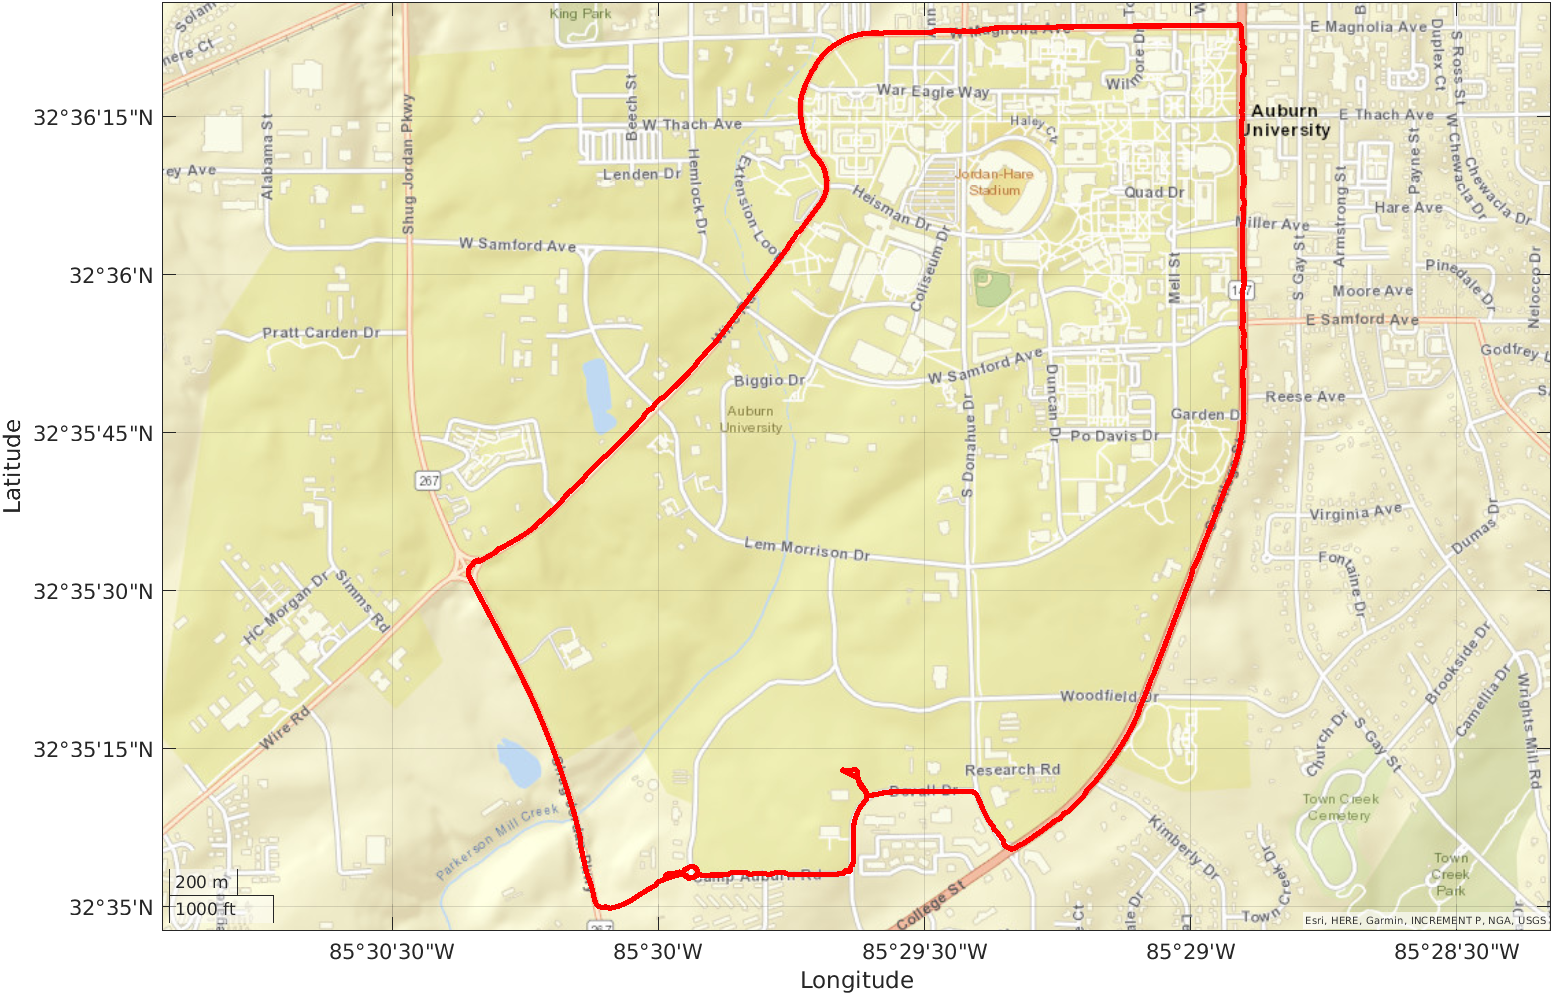
\includegraphics[width=0.7\textwidth]{dynamic_pos.png}
    \caption{Dynamic Receiver Path.}
  \end{figure}
  Note that four timestamps had erroneous data where there were fewer than four 
  satellites in view. These data points were removed from the solution. 
  The data was taken on the streets around Auburn's campus. The path begins 
  and ends at the Auburn MRI building parking lot.\\

  Below is a plot of the DOPs for this dynamic data:
  \begin{figure}[H]
    \centering
    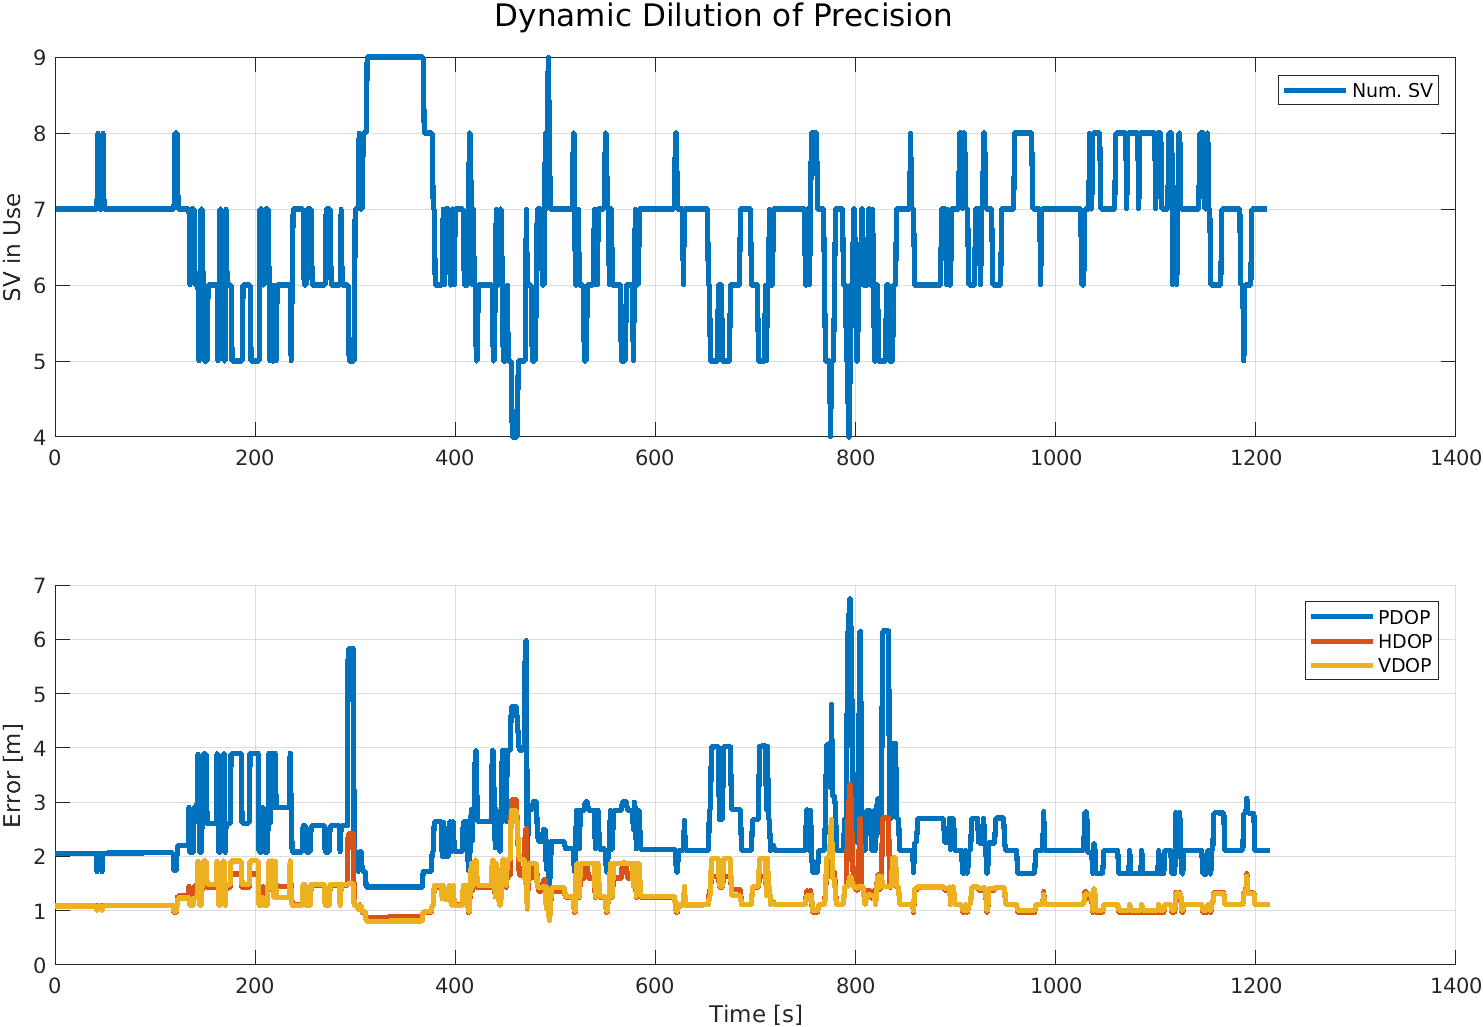
\includegraphics[width=0.7\textwidth]{dynamic_dop.png}
    \caption{Dilution of Precision for the Dynamic Receiver.}
  \end{figure}
  The PDOP shows that the position error could remain below 7 meters at all 
  time points and has a direct correlation to the number of available satellites. 
  Because the data is dynamic, satellites fall out of view more often so the number 
  of satellites in use is much more sporadic.

  The plots for speed and course are shown below:
  \begin{figure}[H]
    \centering
    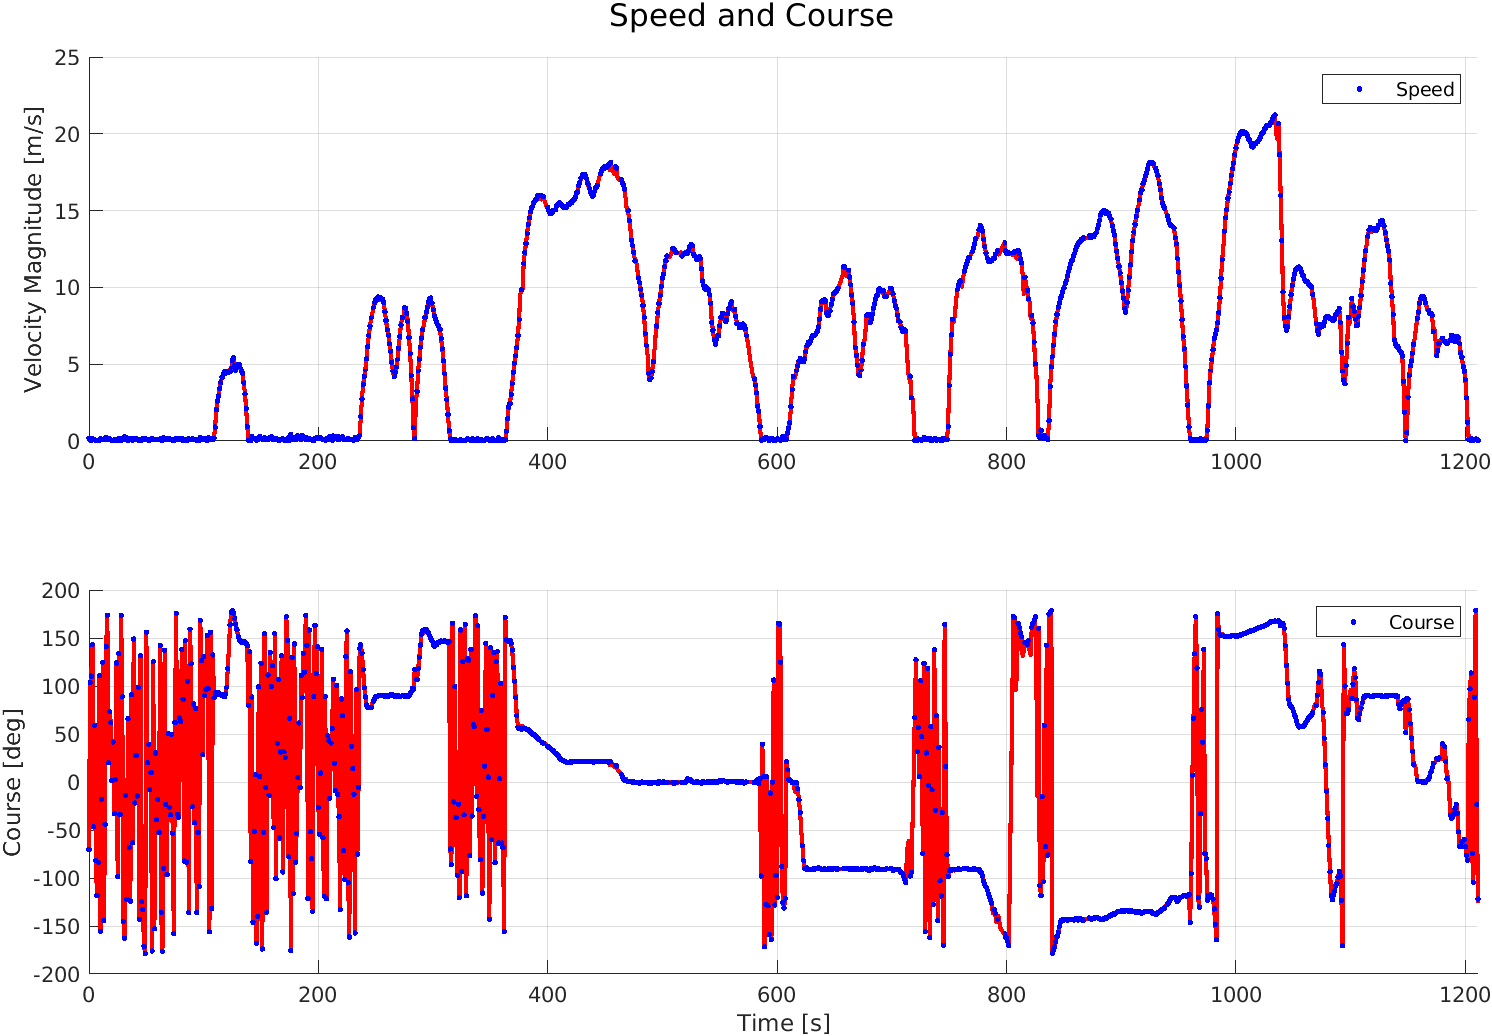
\includegraphics[width=0.7\textwidth]{dynamic_vel_course.png}
    \caption{Speed and Course of Receiver.}
  \end{figure}
  The velocity had many erroneous spikes (of extremly high velocity) caused by bad 
  doppler measurements. Therefore, any velocities over 58 mph ($\sim$26 m/s) were discarded 
  as shown by the blue line. The spaces between these points were linearly interpolated 
  to fill in the gaps as shown by the red line. After correcting this, the velocities 
  never went above about 45 mph. The course was then calculated as a function of the east and 
  north velocities. The graph of course looks as expected with a clear path while moving, 
  and noisy values while stopped. \\

  The clock bias and drift are plotted below:
  \begin{figure}[H]
    \centering
    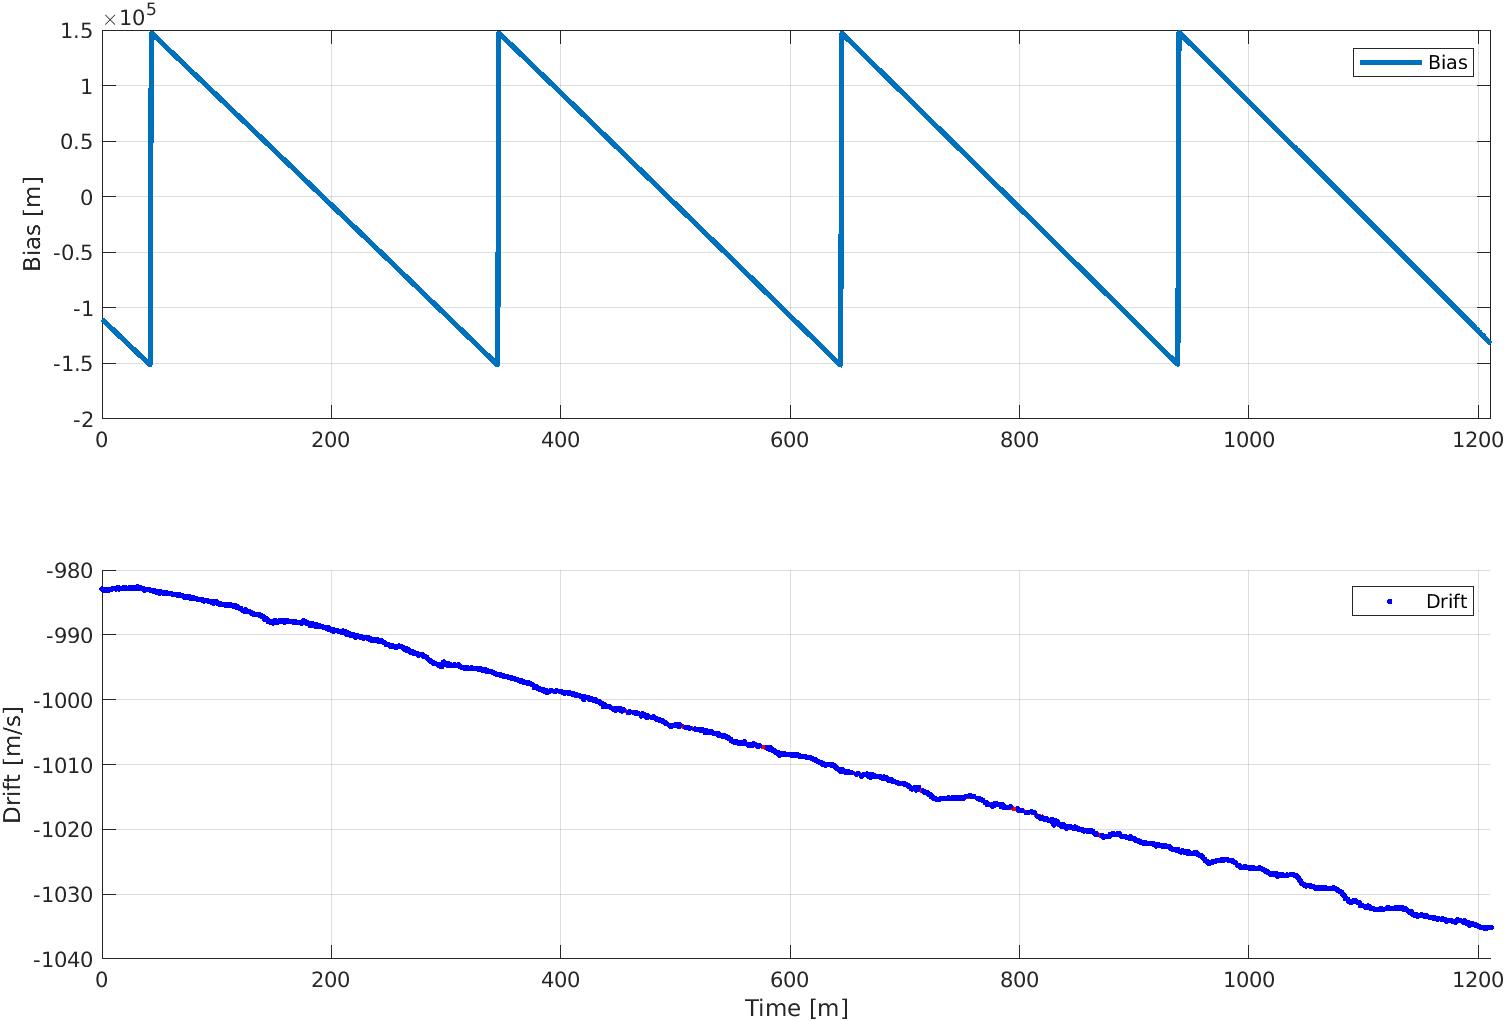
\includegraphics[width=0.7\textwidth]{dynamic_clock.png}
    \caption{Clock Bias and Drift.}
  \end{figure}
  The clock bias constantly decreases to $-1.5(10^5)$ where is gets wrapped back 
  around to $+1.5(10^5)$. If you were to plot the raw pseudoranges for this data 
  set they follow this same pattern. The clock drift (another function of velocity) 
  was also filtered by the removing the points of high velocities and interpolating 
  in the gaps. As shown, it increases in magnitude over time, which is to be expected 
  due to poor doppler measurements degrading the solution.

  \item Bonus from LAB 1.
  \begin{enumerate}[(a)]
    \itemsep = -2pt
    \item Get Ephemerides Online. Using the RINEX files described in class, determine
    the navigation message file that will contain the appropriate parameters to
    calculate the satellite positions. Describe the parts of the filename that indicate
    this is the correct file. You may also be able to get the ephemeris from other
    websites in a more direct form.
    \item Sky View Plot. In terms of GPS week and seconds of week, when are the
    positions to be calculated? Generate the polar sky plot shown in Lab 1 –
    Geocaching and compare to the Sky Plot from Lab 1.
  \end{enumerate}
  \solution 
  A rinex file for January 31, 2023 at UTC time 17:21:27 was downloaded from 
  \url{https://cddis.nasa.gov/archive/gnss/data/hourly/2023/031/17/}. A file 
  from this link was chosen because it provided the closest ephemeris time to 
  the actual time of the measurement. The ephemeris time provided in the rinex 
  file was 2023/01/31 17:06:21, 15 minutes before our collection. The filename 
  (AMC400USA\_R\_20230311600\_01H\_GN.rnx) provides an approximate location with the 
  USA flag, the date given as a string of numbers, as well as GN at the end 
  signifying it contains GPS navigation data. Below are skyplots from 
  \url{http://gnssmissionplanning.com} as well as the one generated with this 
  acquired ephemeris data.
  \begin{figure}[H]
    \centering
    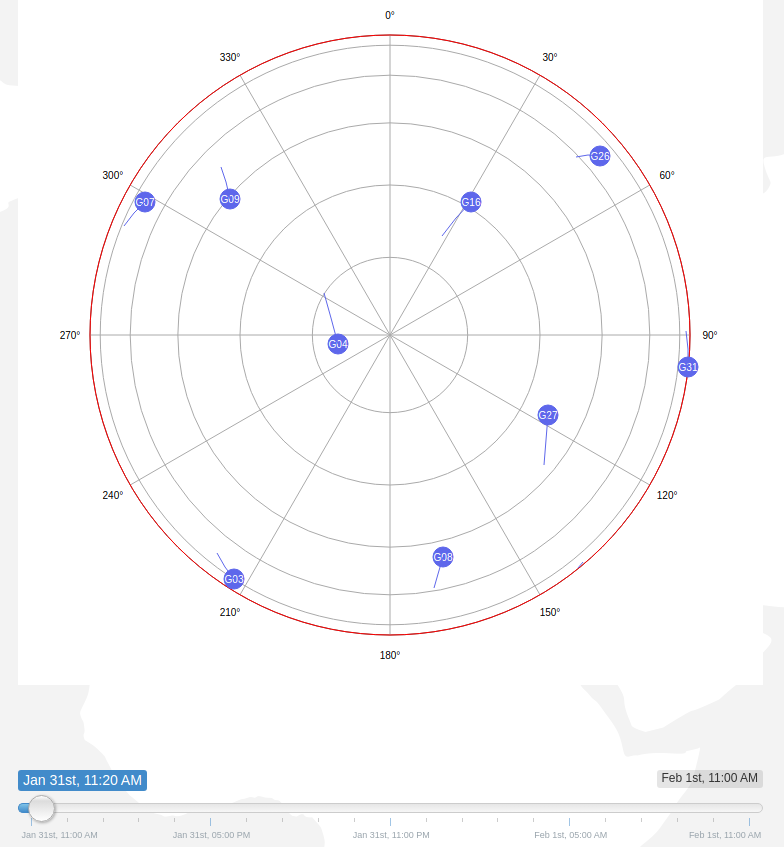
\includegraphics[width=0.55\textwidth]{mission_sky_1120.png}
    \caption{Skyplot from GNSSMissionPlanning}
  \end{figure}
  \begin{figure}[H]
    \centering
    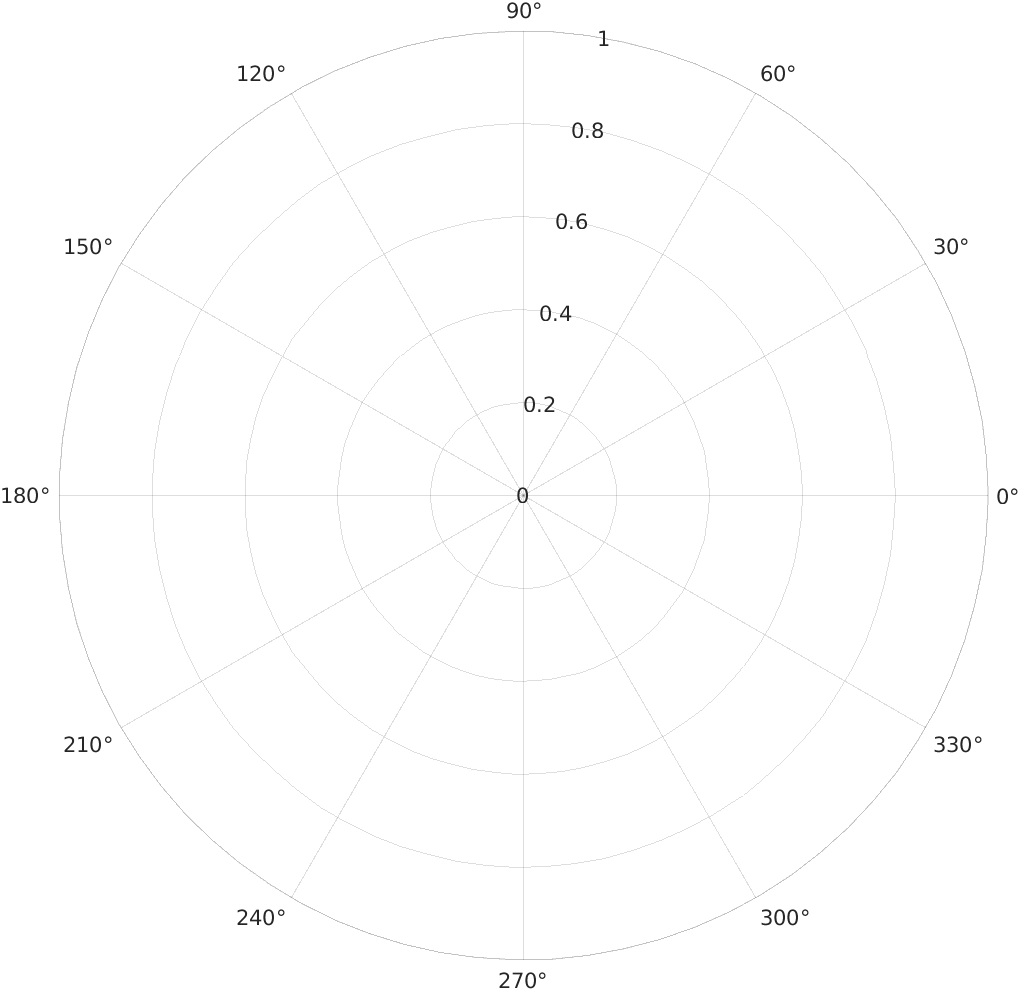
\includegraphics[width=0.55\textwidth]{lab1_skyplot.png}
    \caption{Recreated Skyplot.}
  \end{figure}
  The recreated skyplot was taken at GPS week 2247 and GPS seconds 148887. 
  Both skyplots show the same satellites, however satellite 31 was at a 0 
  degree elevation angle in the skyplot from GNSSMissionPlanning. This same 
  satellite does not appear in the recreated skyplot because the satellites 
  are not in the same positions. The positions of all of the satellites are 
  shifted in the recreated skyplot. This is likely due a discrepancy between 
  the downloaded ephemeris and the GNSSMissionPlanning ephemeris.
\end{enumerate}
\end{document}